\documentclass[10pt]{article}
\usepackage[utf8]{inputenc}
\usepackage[doublespacing]{setspace}
\usepackage{textcomp}
\usepackage{amsmath,amssymb,amsthm}
\usepackage{fancyhdr}
\usepackage{lastpage}
\usepackage[]{hyperref}
\usepackage[pdftex]{graphicx}
\usepackage{ctex}
\usepackage{booktabs}
\usepackage{subfigure}
\usepackage{titlesec}
\usepackage{listings}
\usepackage{enumerate}
\usepackage{bm}
\usepackage{float}
\usepackage{url}
\usepackage[english]{babel}
\usepackage{tikz}
\usepackage{tikz-network}
\usetikzlibrary{arrows.meta,positioning}
\usepackage[margin=1.25in]{geometry}
\usepackage{comment}
%\allowdisplaybreaks
\renewcommand{\contentsname}{\centerline{Contents}}
\pagestyle{fancy}
\author{D}
\def\name{D}
\lhead{Big Data}
\chead{}
\rhead{\name}
\cfoot{-\space\thepage\space-}
\newtheorem{exer}{\bm{$Exercise$}}
\newtheorem{prob}{\bm{$Problem$}}
\newtheorem{bonus}{\bm{$Bonus\;Problem$}}
\newcommand{\tabincell}[2]{\begin{tabular}{@{}#1@{}}#2\end{tabular}}
\CTEXoptions[today=old]

\begin{document}

\title{Assignment Three\\
       \large Part A}
\date{\today}
\maketitle
\thispagestyle{fancy}
\vspace{6mm}

\noindent\textbf{\textit{Problem 1.}}
\begin{enumerate}[1)]
\vspace{3mm}

\item
Given the description of the network, first of all we draw its structure.\\
\begin{figure}[H]
\centering
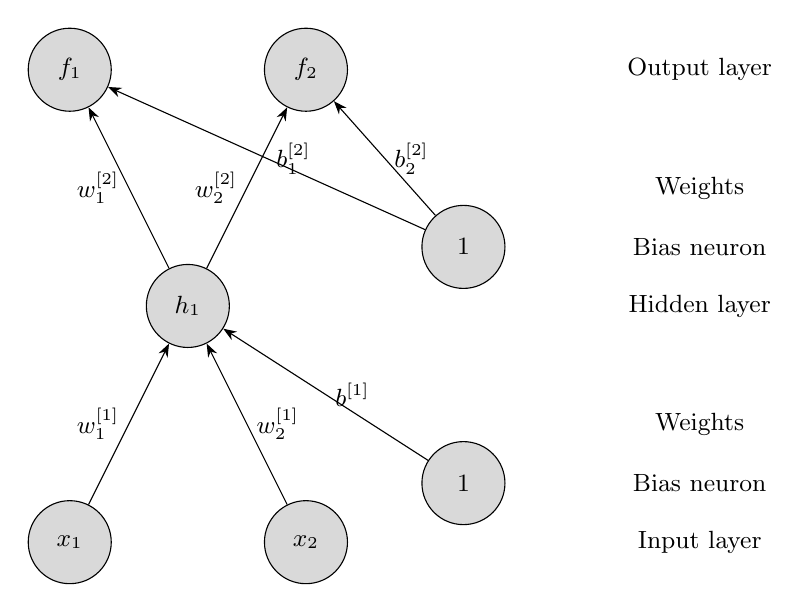
\begin{tikzpicture}[
      mycircle/.style={
         circle,
         draw=black,
         fill=gray,
         fill opacity=0.3,
         text opacity=1,
         inner sep=0pt,
         minimum size=30pt,
         font=\small},
      mytext/.style={
         rectangle,
         font=\small},
      myarrow/.style={-Stealth},
      node distance=1.2cm and 2.4cm
      ]
      \node[mycircle] (c1)at (0,0) {$x_1$};
      \node[mycircle] (c2)at (3,0) {$x_2$};
      \node[mycircle] (c4)at (5,0.75) {$1$};
      \node[mycircle] (c5)at (1.5,3) {$h_1$};;
      \node[mycircle] (c8)at (5,3.75) {$1$};
      \node[mycircle] (c9)at (0,6) {$f_1$};
      \node[mycircle] (c10)at (3,6) {$f_2$};
      \node[mytext] (c21) at (8,0) {Input layer};
      \node[mytext] (c21) at (8,0.75) {Bias neuron};
      \node[mytext] (c21) at (8,1.5) {Weights};
      \node[mytext] (c22) at (8,3) {Hidden layer};
      \node[mytext] (c21) at (8,3.75) {Bias neuron};
      \node[mytext] (c21) at (8,4.5) {Weights};
      \node[mytext] (c21) at (8,6) {Output layer};
    \foreach \i/\j/\txt/\p in {
      c1/c5/$w^{[1]}_{1}$/left,
      c2/c5/$w^{[1]}_{2}$/right,
      c4/c5/$b^{[1]}$/right,
      c5/c9/$w^{[2]}_{1}$/left,
      c5/c10/$w^{[2]}_{2}$/left,
      c8/c9/$b^{[2]}_1$/right,
      c8/c10/$b^{[2]}_2$/right}
       \draw [myarrow] (\i) -- node[font=\small,\p] {\txt} (\j);
\end{tikzpicture}
\caption{Structure of the network}
\end{figure}
Using the given values and functions, we get the complete network.\\
\begin{figure}[H]
\centering
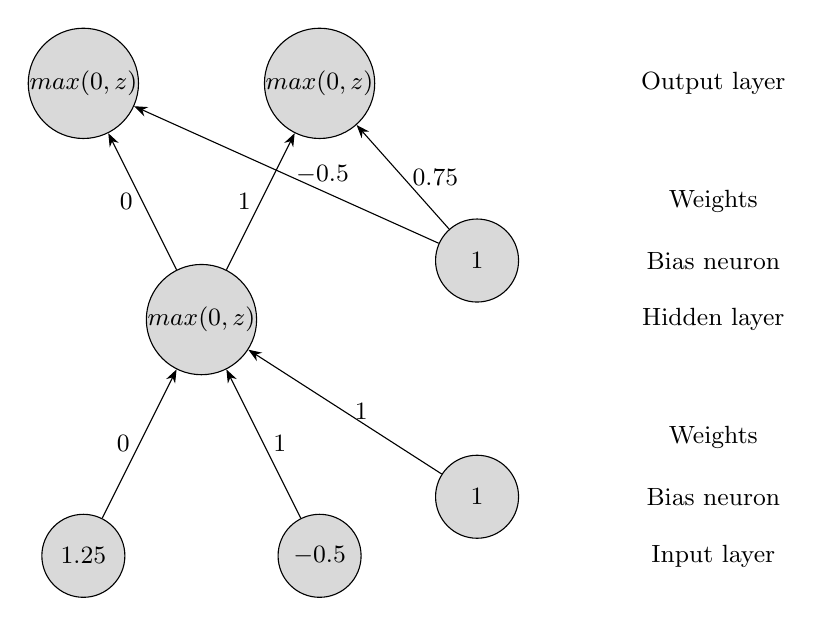
\begin{tikzpicture}[
      mycircle/.style={
         circle,
         draw=black,
         fill=gray,
         fill opacity=0.3,
         text opacity=1,
         inner sep=0pt,
         minimum size=30pt,
         font=\small},
      mytext/.style={
         rectangle,
         font=\small},
      myarrow/.style={-Stealth},
      node distance=1.2cm and 2.4cm
      ]
      \node[mycircle] (c1)at (0,0) {$1.25$};
      \node[mycircle] (c2)at (3,0) {$-0.5$};
      \node[mycircle] (c4)at (5,0.75) {$1$};
      \node[mycircle] (c5)at (1.5,3) {$max(0,z)$};;
      \node[mycircle] (c8)at (5,3.75) {$1$};
      \node[mycircle] (c9)at (0,6) {$max(0,z)$};
      \node[mycircle] (c10)at (3,6) {$max(0,z)$};
      \node[mytext] (c21) at (8,0) {Input layer};
      \node[mytext] (c21) at (8,0.75) {Bias neuron};
      \node[mytext] (c21) at (8,1.5) {Weights};
      \node[mytext] (c22) at (8,3) {Hidden layer};
      \node[mytext] (c21) at (8,3.75) {Bias neuron};
      \node[mytext] (c21) at (8,4.5) {Weights};
      \node[mytext] (c21) at (8,6) {Output layer};
    \foreach \i/\j/\txt/\p in {
      c1/c5/$0$/left,
      c2/c5/$1$/right,
      c4/c5/$1$/right,
      c5/c9/$0$/left,
      c5/c10/$1$/left,
      c8/c9/$-0.5$/right,
      c8/c10/$0.75$/right}
       \draw [myarrow] (\i) -- node[font=\small,\p] {\txt} (\j);
\end{tikzpicture}
\caption{Complete network}
\end{figure}
Then we compute the outputs. We get the sum $z$ in the hidden layer,
\begin{align*}
\pmb{z}&=\pmb{W}^{[1]}\pmb{X}+\pmb{b}^{[1]}\\
&=
  \begin{bmatrix}
    0 & 1
  \end{bmatrix}
  \begin{bmatrix}
    1.25\\
    -0.5
  \end{bmatrix}
+
  \begin{bmatrix}
    1
  \end{bmatrix}\\
&=
  \begin{bmatrix}
    -0.5
  \end{bmatrix}
+
  \begin{bmatrix}
    1
  \end{bmatrix}\\
&=
  \begin{bmatrix}
    0.5
  \end{bmatrix}.
\end{align*}
Input the sum into the activation function and get the outputs $\pmb{h}$ in the hidden layer,
\begin{align*}
\pmb{h}&=g(\pmb{z})\\
&=
  \begin{bmatrix}
    max(0,0.5)\\
  \end{bmatrix}\\
&=
  \begin{bmatrix}
    0.5
  \end{bmatrix}.
\end{align*}
Repeat the process and get the sum $\pmb{z}'$ in the output layer,
\begin{align*}
\pmb{z}'&=\pmb{W}^{[2]}\pmb{h}+\pmb{b}^{[2]}\\
&=
  \begin{bmatrix}
    0\\
    1
  \end{bmatrix}
  \begin{bmatrix}
    0.5
  \end{bmatrix}
+
  \begin{bmatrix}
    -0.5\\
    0.75
  \end{bmatrix}\\
&=
  \begin{bmatrix}
    0\\
    0.5
  \end{bmatrix}
+
  \begin{bmatrix}
    -0.5\\
    0.75
  \end{bmatrix}\\
&=
  \begin{bmatrix}
    -0.5\\
    1.25
  \end{bmatrix}.
\end{align*}
Finally input the sum into the activation function and get the final output $\pmb{f}$,
\begin{align*}
\pmb{f}&=g(\pmb{z}')\\
&=
  \begin{bmatrix}
    max(0,-0.5)\\
    max(0,1.25)
  \end{bmatrix}\\
&=
  \begin{bmatrix}
    0\\
    1.25
  \end{bmatrix}.
\end{align*}
The dimensions of the output are 2. The output is $
  \begin{bmatrix}
    0 & 1.25
  \end{bmatrix}
^{\top}$.\\

\item
Straightforwardly, we apply the filters $F_1$, $F_2$ and $F_3$ to the input image $I$ with a stride of 1 and no padding. Let $O_1$, $O_2$ and $O_3$ be the output feature maps respectively, and we have
\begin{align*}
&O_1=
  \begin{bmatrix}
    1 & 0 & 1\\
    1 & 1 & 1\\
    1 & 1 & 1
  \end{bmatrix}
,\\
&O_2=
  \begin{bmatrix}
    0 & 0 & 0\\
    0 & 0 & 0\\
    0 & 0 & 0
  \end{bmatrix}
,\\
&O_3=
  \begin{bmatrix}
    4 & -3 & 4\\
    2 & 2 & 2\\
    3 & 2 & 3
  \end{bmatrix}
.
\end{align*}
Especially, we plot the following diagrams to show the links between the input and the bottom right pixel of output feature maps through this convolution.\\
\begin{figure}[H]
\centering
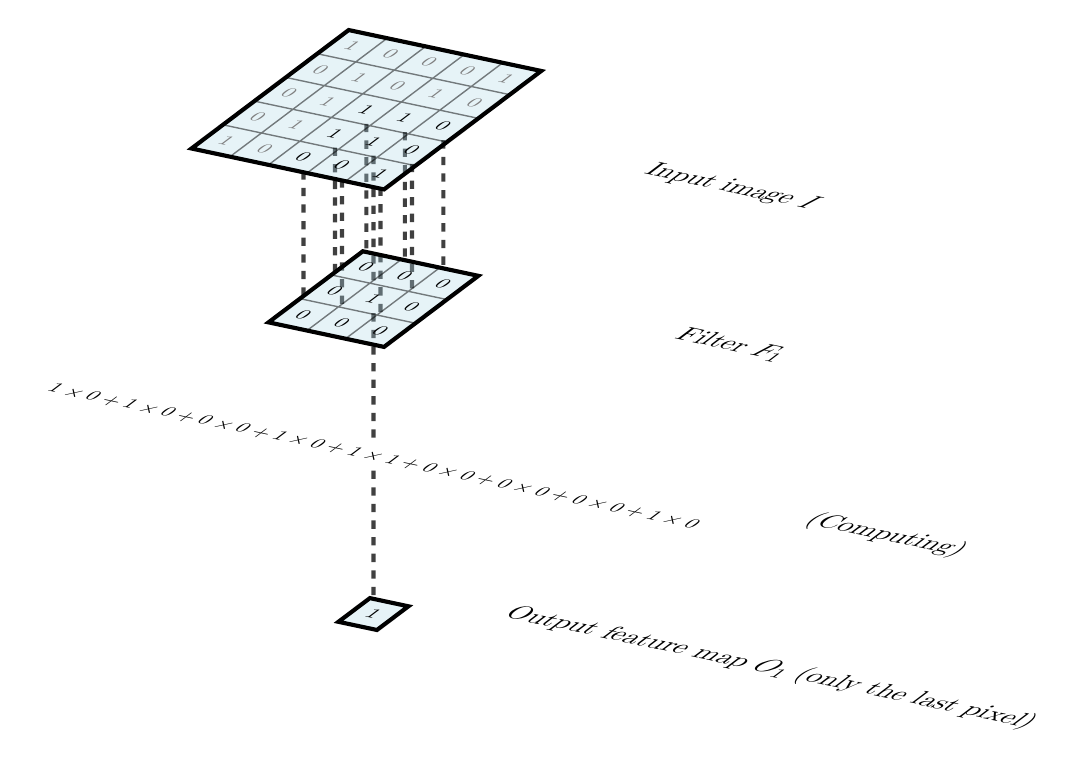
\begin{tikzpicture}[multilayer=3d]
  \Plane[x=0,y=0,width=2.5,height=2.5,grid=5mm,layer=1]
  \Plane[x=1,y=0,width=1.5,height=1.5,grid=5mm,layer=2]
  \Plane[x=1.5,y=0.5,width=0.5,height=0.5,grid=5mm,layer=4]
  \Vertex[x=0.25,y=0.25,layer=1,label=1,fontcolor=gray,style={color=white,opacity=0}]{}
  \Vertex[x=0.75,y=0.25,layer=1,label=0,fontcolor=gray,style={color=white,opacity=0}]{}
  \Vertex[x=1.25,y=0.25,layer=1,label=0,style={color=white,opacity=0}]{I1}
  \Vertex[x=1.75,y=0.25,layer=1,label=0,style={color=white,opacity=0}]{I2}
  \Vertex[x=2.25,y=0.25,layer=1,label=1,style={color=white,opacity=0}]{I3}
  \Vertex[x=0.25,y=0.75,layer=1,label=0,fontcolor=gray,style={color=white,opacity=0}]{}
  \Vertex[x=0.75,y=0.75,layer=1,label=1,fontcolor=gray,style={color=white,opacity=0}]{}
  \Vertex[x=1.25,y=0.75,layer=1,label=1,style={color=white,opacity=0}]{I4}
  \Vertex[x=1.75,y=0.75,layer=1,label=1,style={color=white,opacity=0}]{I5}
  \Vertex[x=2.25,y=0.75,layer=1,label=0,style={color=white,opacity=0}]{I6}
  \Vertex[x=0.25,y=1.25,layer=1,label=0,fontcolor=gray,style={color=white,opacity=0}]{}
  \Vertex[x=0.75,y=1.25,layer=1,label=1,fontcolor=gray,style={color=white,opacity=0}]{}
  \Vertex[x=1.25,y=1.25,layer=1,label=1,style={color=white,opacity=0}]{I7}
  \Vertex[x=1.75,y=1.25,layer=1,label=1,style={color=white,opacity=0}]{I8}
  \Vertex[x=2.25,y=1.25,layer=1,label=0,style={color=white,opacity=0}]{I9}
  \Vertex[x=0.25,y=1.75,layer=1,label=0,fontcolor=gray,style={color=white,opacity=0}]{}
  \Vertex[x=0.75,y=1.75,layer=1,label=1,fontcolor=gray,style={color=white,opacity=0}]{}
  \Vertex[x=1.25,y=1.75,layer=1,label=0,fontcolor=gray,style={color=white,opacity=0}]{}
  \Vertex[x=1.75,y=1.75,layer=1,label=1,fontcolor=gray,style={color=white,opacity=0}]{}
  \Vertex[x=2.25,y=1.75,layer=1,label=0,fontcolor=gray,style={color=white,opacity=0}]{}
  \Vertex[x=0.25,y=2.25,layer=1,label=1,fontcolor=gray,style={color=white,opacity=0}]{}
  \Vertex[x=0.75,y=2.25,layer=1,label=0,fontcolor=gray,style={color=white,opacity=0}]{}
  \Vertex[x=1.25,y=2.25,layer=1,label=0,fontcolor=gray,style={color=white,opacity=0}]{}
  \Vertex[x=1.75,y=2.25,layer=1,label=0,fontcolor=gray,style={color=white,opacity=0}]{}
  \Vertex[x=2.25,y=2.25,layer=1,label=1,fontcolor=gray,style={color=white,opacity=0}]{}
  \Text[x=6,y=1.25,layer=1]{Input image $I$}
  \Vertex[x=1.25,y=0.25,layer=2,label=0,style={color=white,opacity=0}]{F1}
  \Vertex[x=1.75,y=0.25,layer=2,label=0,style={color=white,opacity=0}]{F2}
  \Vertex[x=2.25,y=0.25,layer=2,label=0,style={color=white,opacity=0}]{F3}
  \Vertex[x=1.25,y=0.75,layer=2,label=0,style={color=white,opacity=0}]{F4}
  \Vertex[x=1.75,y=0.75,layer=2,label=1,style={color=white,opacity=0}]{F5}
  \Vertex[x=2.25,y=0.75,layer=2,label=0,style={color=white,opacity=0}]{F6}
  \Vertex[x=1.25,y=1.25,layer=2,label=0,style={color=white,opacity=0}]{F7}
  \Vertex[x=1.75,y=1.25,layer=2,label=0,style={color=white,opacity=0}]{F8}
  \Vertex[x=2.25,y=1.25,layer=2,label=0,style={color=white,opacity=0}]{F9}
  \Text[x=6,y=1.25,layer=2]{Filter $F_1$}
  \Edge[style={dashed}](I1)(F1)
  \Edge[style={dashed}](I2)(F2)
  \Edge[style={dashed}](I3)(F3)
  \Edge[style={dashed}](I4)(F4)
  \Edge[style={dashed}](I5)(F5)
  \Edge[style={dashed}](I6)(F6)
  \Edge[style={dashed}](I7)(F7)
  \Edge[style={dashed}](I8)(F8)
  \Edge[style={dashed}](I9)(F9)
  \Vertex[x=1.75,y=0.75,layer=3,label=$1\times0+1\times0+0\times0+1\times0+1\times1+0\times0+0\times0+0\times0+1\times0$,style={color=white,opacity=0}]{C}
  \Text[x=8,y=1.25,layer=3]{(Computing)}
  \Edge[style={dashed}](F5)(C)
  \Vertex[x=1.75,y=0.75,layer=4,label=1,style={color=white,opacity=0}]{O}
  \Text[x=6.5,y=1.25,layer=4]{Output feature map $O_1$ (only the last pixel)}
  \Edge[style={dashed}](C)(O)
\end{tikzpicture}
\caption{Link between $I$ and the bottom right pixel of $O_1$}
\end{figure}
\begin{figure}[H]
\centering
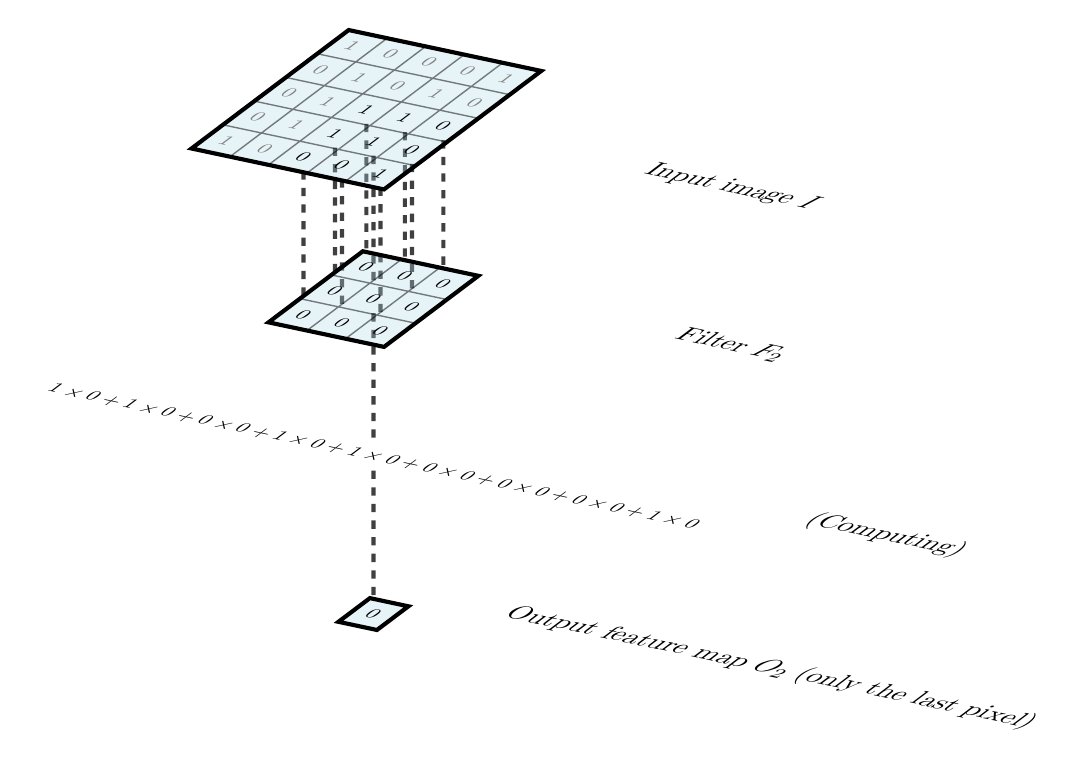
\begin{tikzpicture}[multilayer=3d]
  \Plane[x=0,y=0,width=2.5,height=2.5,grid=5mm,layer=1]
  \Plane[x=1,y=0,width=1.5,height=1.5,grid=5mm,layer=2]
  \Plane[x=1.5,y=0.5,width=0.5,height=0.5,grid=5mm,layer=4]
  \Vertex[x=0.25,y=0.25,layer=1,label=1,fontcolor=gray,style={color=white,opacity=0}]{}
  \Vertex[x=0.75,y=0.25,layer=1,label=0,fontcolor=gray,style={color=white,opacity=0}]{}
  \Vertex[x=1.25,y=0.25,layer=1,label=0,style={color=white,opacity=0}]{I1}
  \Vertex[x=1.75,y=0.25,layer=1,label=0,style={color=white,opacity=0}]{I2}
  \Vertex[x=2.25,y=0.25,layer=1,label=1,style={color=white,opacity=0}]{I3}
  \Vertex[x=0.25,y=0.75,layer=1,label=0,fontcolor=gray,style={color=white,opacity=0}]{}
  \Vertex[x=0.75,y=0.75,layer=1,label=1,fontcolor=gray,style={color=white,opacity=0}]{}
  \Vertex[x=1.25,y=0.75,layer=1,label=1,style={color=white,opacity=0}]{I4}
  \Vertex[x=1.75,y=0.75,layer=1,label=1,style={color=white,opacity=0}]{I5}
  \Vertex[x=2.25,y=0.75,layer=1,label=0,style={color=white,opacity=0}]{I6}
  \Vertex[x=0.25,y=1.25,layer=1,label=0,fontcolor=gray,style={color=white,opacity=0}]{}
  \Vertex[x=0.75,y=1.25,layer=1,label=1,fontcolor=gray,style={color=white,opacity=0}]{}
  \Vertex[x=1.25,y=1.25,layer=1,label=1,style={color=white,opacity=0}]{I7}
  \Vertex[x=1.75,y=1.25,layer=1,label=1,style={color=white,opacity=0}]{I8}
  \Vertex[x=2.25,y=1.25,layer=1,label=0,style={color=white,opacity=0}]{I9}
  \Vertex[x=0.25,y=1.75,layer=1,label=0,fontcolor=gray,style={color=white,opacity=0}]{}
  \Vertex[x=0.75,y=1.75,layer=1,label=1,fontcolor=gray,style={color=white,opacity=0}]{}
  \Vertex[x=1.25,y=1.75,layer=1,label=0,fontcolor=gray,style={color=white,opacity=0}]{}
  \Vertex[x=1.75,y=1.75,layer=1,label=1,fontcolor=gray,style={color=white,opacity=0}]{}
  \Vertex[x=2.25,y=1.75,layer=1,label=0,fontcolor=gray,style={color=white,opacity=0}]{}
  \Vertex[x=0.25,y=2.25,layer=1,label=1,fontcolor=gray,style={color=white,opacity=0}]{}
  \Vertex[x=0.75,y=2.25,layer=1,label=0,fontcolor=gray,style={color=white,opacity=0}]{}
  \Vertex[x=1.25,y=2.25,layer=1,label=0,fontcolor=gray,style={color=white,opacity=0}]{}
  \Vertex[x=1.75,y=2.25,layer=1,label=0,fontcolor=gray,style={color=white,opacity=0}]{}
  \Vertex[x=2.25,y=2.25,layer=1,label=1,fontcolor=gray,style={color=white,opacity=0}]{}
  \Text[x=6,y=1.25,layer=1]{Input image $I$}
  \Vertex[x=1.25,y=0.25,layer=2,label=0,style={color=white,opacity=0}]{F1}
  \Vertex[x=1.75,y=0.25,layer=2,label=0,style={color=white,opacity=0}]{F2}
  \Vertex[x=2.25,y=0.25,layer=2,label=0,style={color=white,opacity=0}]{F3}
  \Vertex[x=1.25,y=0.75,layer=2,label=0,style={color=white,opacity=0}]{F4}
  \Vertex[x=1.75,y=0.75,layer=2,label=0,style={color=white,opacity=0}]{F5}
  \Vertex[x=2.25,y=0.75,layer=2,label=0,style={color=white,opacity=0}]{F6}
  \Vertex[x=1.25,y=1.25,layer=2,label=0,style={color=white,opacity=0}]{F7}
  \Vertex[x=1.75,y=1.25,layer=2,label=0,style={color=white,opacity=0}]{F8}
  \Vertex[x=2.25,y=1.25,layer=2,label=0,style={color=white,opacity=0}]{F9}
  \Text[x=6,y=1.25,layer=2]{Filter $F_2$}
  \Edge[style={dashed}](I1)(F1)
  \Edge[style={dashed}](I2)(F2)
  \Edge[style={dashed}](I3)(F3)
  \Edge[style={dashed}](I4)(F4)
  \Edge[style={dashed}](I5)(F5)
  \Edge[style={dashed}](I6)(F6)
  \Edge[style={dashed}](I7)(F7)
  \Edge[style={dashed}](I8)(F8)
  \Edge[style={dashed}](I9)(F9)
  \Vertex[x=1.75,y=0.75,layer=3,label=$1\times0+1\times0+0\times0+1\times0+1\times0+0\times0+0\times0+0\times0+1\times0$,style={color=white,opacity=0}]{C}
  \Text[x=8,y=1.25,layer=3]{(Computing)}
  \Edge[style={dashed}](F5)(C)
  \Vertex[x=1.75,y=0.75,layer=4,label=0,style={color=white,opacity=0}]{O}
  \Text[x=6.5,y=1.25,layer=4]{Output feature map $O_2$ (only the last pixel)}
  \Edge[style={dashed}](C)(O)
\end{tikzpicture}
\caption{Link between $I$ and the bottom right pixel of $O_2$}
\end{figure}
\begin{figure}[H]
\centering
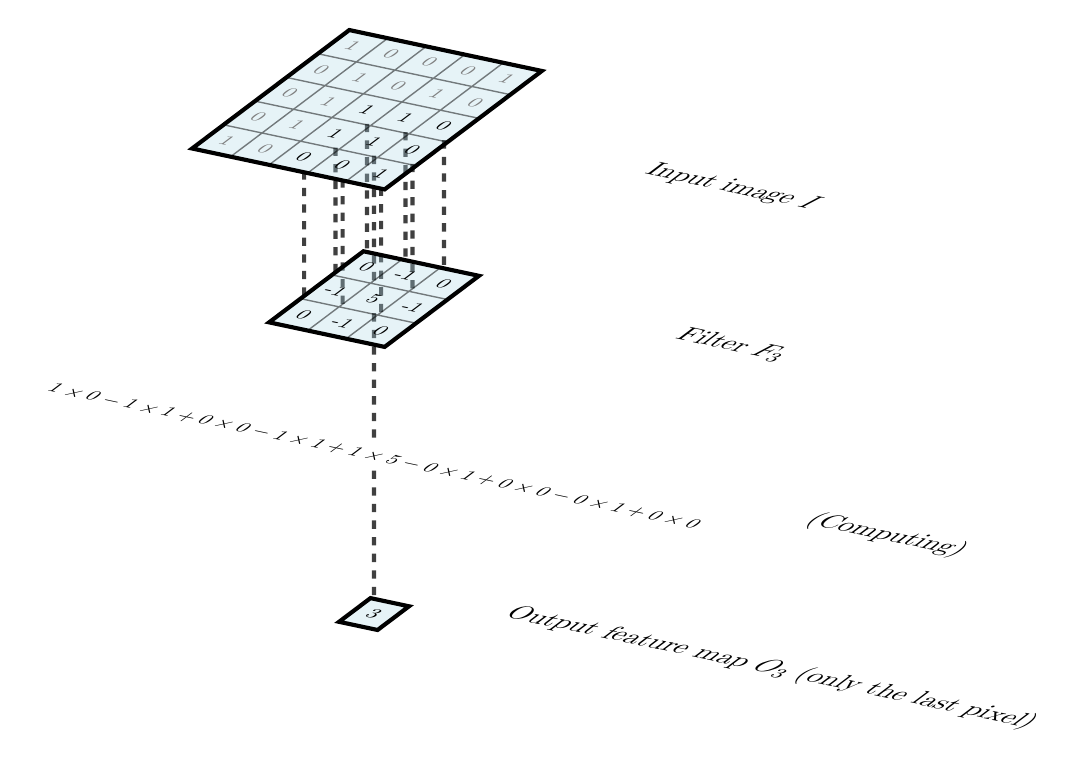
\begin{tikzpicture}[multilayer=3d]
  \Plane[x=0,y=0,width=2.5,height=2.5,grid=5mm,layer=1]
  \Plane[x=1,y=0,width=1.5,height=1.5,grid=5mm,layer=2]
  \Plane[x=1.5,y=0.5,width=0.5,height=0.5,grid=5mm,layer=4]
  \Vertex[x=0.25,y=0.25,layer=1,label=1,fontcolor=gray,style={color=white,opacity=0}]{}
  \Vertex[x=0.75,y=0.25,layer=1,label=0,fontcolor=gray,style={color=white,opacity=0}]{}
  \Vertex[x=1.25,y=0.25,layer=1,label=0,style={color=white,opacity=0}]{I1}
  \Vertex[x=1.75,y=0.25,layer=1,label=0,style={color=white,opacity=0}]{I2}
  \Vertex[x=2.25,y=0.25,layer=1,label=1,style={color=white,opacity=0}]{I3}
  \Vertex[x=0.25,y=0.75,layer=1,label=0,fontcolor=gray,style={color=white,opacity=0}]{}
  \Vertex[x=0.75,y=0.75,layer=1,label=1,fontcolor=gray,style={color=white,opacity=0}]{}
  \Vertex[x=1.25,y=0.75,layer=1,label=1,style={color=white,opacity=0}]{I4}
  \Vertex[x=1.75,y=0.75,layer=1,label=1,style={color=white,opacity=0}]{I5}
  \Vertex[x=2.25,y=0.75,layer=1,label=0,style={color=white,opacity=0}]{I6}
  \Vertex[x=0.25,y=1.25,layer=1,label=0,fontcolor=gray,style={color=white,opacity=0}]{}
  \Vertex[x=0.75,y=1.25,layer=1,label=1,fontcolor=gray,style={color=white,opacity=0}]{}
  \Vertex[x=1.25,y=1.25,layer=1,label=1,style={color=white,opacity=0}]{I7}
  \Vertex[x=1.75,y=1.25,layer=1,label=1,style={color=white,opacity=0}]{I8}
  \Vertex[x=2.25,y=1.25,layer=1,label=0,style={color=white,opacity=0}]{I9}
  \Vertex[x=0.25,y=1.75,layer=1,label=0,fontcolor=gray,style={color=white,opacity=0}]{}
  \Vertex[x=0.75,y=1.75,layer=1,label=1,fontcolor=gray,style={color=white,opacity=0}]{}
  \Vertex[x=1.25,y=1.75,layer=1,label=0,fontcolor=gray,style={color=white,opacity=0}]{}
  \Vertex[x=1.75,y=1.75,layer=1,label=1,fontcolor=gray,style={color=white,opacity=0}]{}
  \Vertex[x=2.25,y=1.75,layer=1,label=0,fontcolor=gray,style={color=white,opacity=0}]{}
  \Vertex[x=0.25,y=2.25,layer=1,label=1,fontcolor=gray,style={color=white,opacity=0}]{}
  \Vertex[x=0.75,y=2.25,layer=1,label=0,fontcolor=gray,style={color=white,opacity=0}]{}
  \Vertex[x=1.25,y=2.25,layer=1,label=0,fontcolor=gray,style={color=white,opacity=0}]{}
  \Vertex[x=1.75,y=2.25,layer=1,label=0,fontcolor=gray,style={color=white,opacity=0}]{}
  \Vertex[x=2.25,y=2.25,layer=1,label=1,fontcolor=gray,style={color=white,opacity=0}]{}
  \Text[x=6,y=1.25,layer=1]{Input image $I$}
  \Vertex[x=1.25,y=0.25,layer=2,label=0,style={color=white,opacity=0}]{F1}
  \Vertex[x=1.75,y=0.25,layer=2,label=-1,style={color=white,opacity=0}]{F2}
  \Vertex[x=2.25,y=0.25,layer=2,label=0,style={color=white,opacity=0}]{F3}
  \Vertex[x=1.25,y=0.75,layer=2,label=-1,style={color=white,opacity=0}]{F4}
  \Vertex[x=1.75,y=0.75,layer=2,label=5,style={color=white,opacity=0}]{F5}
  \Vertex[x=2.25,y=0.75,layer=2,label=-1,style={color=white,opacity=0}]{F6}
  \Vertex[x=1.25,y=1.25,layer=2,label=0,style={color=white,opacity=0}]{F7}
  \Vertex[x=1.75,y=1.25,layer=2,label=-1,style={color=white,opacity=0}]{F8}
  \Vertex[x=2.25,y=1.25,layer=2,label=0,style={color=white,opacity=0}]{F9}
  \Text[x=6,y=1.25,layer=2]{Filter $F_3$}
  \Edge[style={dashed}](I1)(F1)
  \Edge[style={dashed}](I2)(F2)
  \Edge[style={dashed}](I3)(F3)
  \Edge[style={dashed}](I4)(F4)
  \Edge[style={dashed}](I5)(F5)
  \Edge[style={dashed}](I6)(F6)
  \Edge[style={dashed}](I7)(F7)
  \Edge[style={dashed}](I8)(F8)
  \Edge[style={dashed}](I9)(F9)
  \Vertex[x=1.75,y=0.75,layer=3,label=$1\times0-1\times1+0\times0-1\times1+1\times5-0\times1+0\times0-0\times1+0\times0$,style={color=white,opacity=0}]{C}
  \Text[x=8,y=1.25,layer=3]{(Computing)}
  \Edge[style={dashed}](F5)(C)
  \Vertex[x=1.75,y=0.75,layer=4,label=3,style={color=white,opacity=0}]{O}
  \Text[x=6.5,y=1.25,layer=4]{Output feature map $O_3$ (only the last pixel)}
  \Edge[style={dashed}](C)(O)
\end{tikzpicture}
\caption{Link between $I$ and the bottom right pixel of $O_3$}
\end{figure}
\end{enumerate}
\begin{comment}
\begin{figure}[H]
\centering
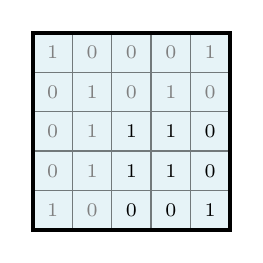
\begin{tikzpicture}
  \Plane[x=0,y=0,width=2.5,height=2.5,grid=5mm]
  \Vertex[x=0.25,y=0.25,label=1,fontcolor=gray,style={color=white,opacity=0}]{}
  \Vertex[x=0.75,y=0.25,label=0,fontcolor=gray,style={color=white,opacity=0}]{}
  \Vertex[x=1.25,y=0.25,label=0,style={color=white,opacity=0}]{I1}
  \Vertex[x=1.75,y=0.25,label=0,style={color=white,opacity=0}]{I2}
  \Vertex[x=2.25,y=0.25,label=1,style={color=white,opacity=0}]{I3}
  \Vertex[x=0.25,y=0.75,label=0,fontcolor=gray,style={color=white,opacity=0}]{}
  \Vertex[x=0.75,y=0.75,label=1,fontcolor=gray,style={color=white,opacity=0}]{}
  \Vertex[x=1.25,y=0.75,label=1,style={color=white,opacity=0}]{I4}
  \Vertex[x=1.75,y=0.75,label=1,style={color=white,opacity=0}]{I5}
  \Vertex[x=2.25,y=0.75,label=0,style={color=white,opacity=0}]{I6}
  \Vertex[x=0.25,y=1.25,label=0,fontcolor=gray,style={color=white,opacity=0}]{}
  \Vertex[x=0.75,y=1.25,label=1,fontcolor=gray,style={color=white,opacity=0}]{}
  \Vertex[x=1.25,y=1.25,label=1,style={color=white,opacity=0}]{I7}
  \Vertex[x=1.75,y=1.25,label=1,style={color=white,opacity=0}]{I8}
  \Vertex[x=2.25,y=1.25,label=0,style={color=white,opacity=0}]{I9}
  \Vertex[x=0.25,y=1.75,label=0,fontcolor=gray,style={color=white,opacity=0}]{}
  \Vertex[x=0.75,y=1.75,label=1,fontcolor=gray,style={color=white,opacity=0}]{}
  \Vertex[x=1.25,y=1.75,label=0,fontcolor=gray,style={color=white,opacity=0}]{}
  \Vertex[x=1.75,y=1.75,label=1,fontcolor=gray,style={color=white,opacity=0}]{}
  \Vertex[x=2.25,y=1.75,label=0,fontcolor=gray,style={color=white,opacity=0}]{}
  \Vertex[x=0.25,y=2.25,label=1,fontcolor=gray,style={color=white,opacity=0}]{}
  \Vertex[x=0.75,y=2.25,label=0,fontcolor=gray,style={color=white,opacity=0}]{}
  \Vertex[x=1.25,y=2.25,label=0,fontcolor=gray,style={color=white,opacity=0}]{}
  \Vertex[x=1.75,y=2.25,label=0,fontcolor=gray,style={color=white,opacity=0}]{}
  \Vertex[x=2.25,y=2.25,label=1,fontcolor=gray,style={color=white,opacity=0}]{}
\end{tikzpicture}
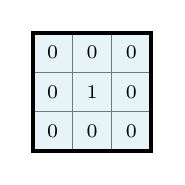
\begin{tikzpicture}
  \Plane[x=1,y=0,width=1.5,height=1.5,grid=5mm]
  \Vertex[x=0.25,y=1.25,label=0,style={color=white,opacity=0}]{F1}
  \Vertex[x=0.75,y=1.25,label=0,style={color=white,opacity=0}]{F2}
  \Vertex[x=1.25,y=1.25,label=0,style={color=white,opacity=0}]{F3}
  \Vertex[x=0.25,y=1.75,label=0,style={color=white,opacity=0}]{F4}
  \Vertex[x=0.75,y=1.75,label=1,style={color=white,opacity=0}]{F5}
  \Vertex[x=1.25,y=1.75,label=0,style={color=white,opacity=0}]{F6}
  \Vertex[x=0.25,y=2.25,label=0,style={color=white,opacity=0}]{F7}
  \Vertex[x=0.75,y=2.25,label=0,style={color=white,opacity=0}]{F8}
  \Vertex[x=1.25,y=2.25,label=0,style={color=white,opacity=0}]{F9}
\end{tikzpicture}
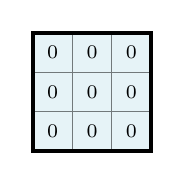
\begin{tikzpicture}
  \Plane[x=1,y=0,width=1.5,height=1.5,grid=5mm]
  \Vertex[x=0.25,y=1.25,label=0,style={color=white,opacity=0}]{F1}
  \Vertex[x=0.75,y=1.25,label=0,style={color=white,opacity=0}]{F2}
  \Vertex[x=1.25,y=1.25,label=0,style={color=white,opacity=0}]{F3}
  \Vertex[x=0.25,y=1.75,label=0,style={color=white,opacity=0}]{F4}
  \Vertex[x=0.75,y=1.75,label=0,style={color=white,opacity=0}]{F5}
  \Vertex[x=1.25,y=1.75,label=0,style={color=white,opacity=0}]{F6}
  \Vertex[x=0.25,y=2.25,label=0,style={color=white,opacity=0}]{F7}
  \Vertex[x=0.75,y=2.25,label=0,style={color=white,opacity=0}]{F8}
  \Vertex[x=1.25,y=2.25,label=0,style={color=white,opacity=0}]{F9}
\end{tikzpicture}
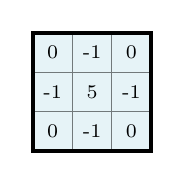
\begin{tikzpicture}
  \Plane[x=1,y=0,width=1.5,height=1.5,grid=5mm]
  \Vertex[x=0.25,y=1.25,label=0,style={color=white,opacity=0}]{F1}
  \Vertex[x=0.75,y=1.25,label=-1,style={color=white,opacity=0}]{F2}
  \Vertex[x=1.25,y=1.25,label=0,style={color=white,opacity=0}]{F3}
  \Vertex[x=0.25,y=1.75,label=-1,style={color=white,opacity=0}]{F4}
  \Vertex[x=0.75,y=1.75,label=5,style={color=white,opacity=0}]{F5}
  \Vertex[x=1.25,y=1.75,label=-1,style={color=white,opacity=0}]{F6}
  \Vertex[x=0.25,y=2.25,label=0,style={color=white,opacity=0}]{F7}
  \Vertex[x=0.75,y=2.25,label=-1,style={color=white,opacity=0}]{F8}
  \Vertex[x=1.25,y=2.25,label=0,style={color=white,opacity=0}]{F9}
\end{tikzpicture}
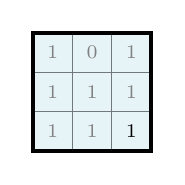
\begin{tikzpicture}
  \Plane[x=1,y=0,width=1.5,height=1.5,grid=5mm]
  \Vertex[x=0.25,y=1.25,label=1,fontcolor=gray,style={color=white,opacity=0}]{F1}
  \Vertex[x=0.75,y=1.25,label=1,fontcolor=gray,style={color=white,opacity=0}]{F2}
  \Vertex[x=1.25,y=1.25,label=1,style={color=white,opacity=0}]{F3}
  \Vertex[x=0.25,y=1.75,label=1,fontcolor=gray,style={color=white,opacity=0}]{F4}
  \Vertex[x=0.75,y=1.75,label=1,fontcolor=gray,style={color=white,opacity=0}]{F5}
  \Vertex[x=1.25,y=1.75,label=1,fontcolor=gray,style={color=white,opacity=0}]{F6}
  \Vertex[x=0.25,y=2.25,label=1,fontcolor=gray,style={color=white,opacity=0}]{F7}
  \Vertex[x=0.75,y=2.25,label=0,fontcolor=gray,style={color=white,opacity=0}]{F8}
  \Vertex[x=1.25,y=2.25,label=1,fontcolor=gray,style={color=white,opacity=0}]{F9}
\end{tikzpicture}
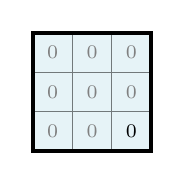
\begin{tikzpicture}
  \Plane[x=1,y=0,width=1.5,height=1.5,grid=5mm]
  \Vertex[x=0.25,y=1.25,label=0,fontcolor=gray,style={color=white,opacity=0}]{F1}
  \Vertex[x=0.75,y=1.25,label=0,fontcolor=gray,style={color=white,opacity=0}]{F2}
  \Vertex[x=1.25,y=1.25,label=0,style={color=white,opacity=0}]{F3}
  \Vertex[x=0.25,y=1.75,label=0,fontcolor=gray,style={color=white,opacity=0}]{F4}
  \Vertex[x=0.75,y=1.75,label=0,fontcolor=gray,style={color=white,opacity=0}]{F5}
  \Vertex[x=1.25,y=1.75,label=0,fontcolor=gray,style={color=white,opacity=0}]{F6}
  \Vertex[x=0.25,y=2.25,label=0,fontcolor=gray,style={color=white,opacity=0}]{F7}
  \Vertex[x=0.75,y=2.25,label=0,fontcolor=gray,style={color=white,opacity=0}]{F8}
  \Vertex[x=1.25,y=2.25,label=0,fontcolor=gray,style={color=white,opacity=0}]{F9}
\end{tikzpicture}
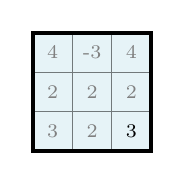
\begin{tikzpicture}
  \Plane[x=1,y=0,width=1.5,height=1.5,grid=5mm]
  \Vertex[x=0.25,y=1.25,label=3,fontcolor=gray,style={color=white,opacity=0}]{F1}
  \Vertex[x=0.75,y=1.25,label=2,fontcolor=gray,style={color=white,opacity=0}]{F2}
  \Vertex[x=1.25,y=1.25,label=3,style={color=white,opacity=0}]{F3}
  \Vertex[x=0.25,y=1.75,label=2,fontcolor=gray,style={color=white,opacity=0}]{F4}
  \Vertex[x=0.75,y=1.75,label=2,fontcolor=gray,style={color=white,opacity=0}]{F5}
  \Vertex[x=1.25,y=1.75,label=2,fontcolor=gray,style={color=white,opacity=0}]{F6}
  \Vertex[x=0.25,y=2.25,label=4,fontcolor=gray,style={color=white,opacity=0}]{F7}
  \Vertex[x=0.75,y=2.25,label=-3,fontcolor=gray,style={color=white,opacity=0}]{F8}
  \Vertex[x=1.25,y=2.25,label=4,fontcolor=gray,style={color=white,opacity=0}]{F9}
\end{tikzpicture}
\end{figure}
\end{comment}
\begin{figure}[H]
  \centering
  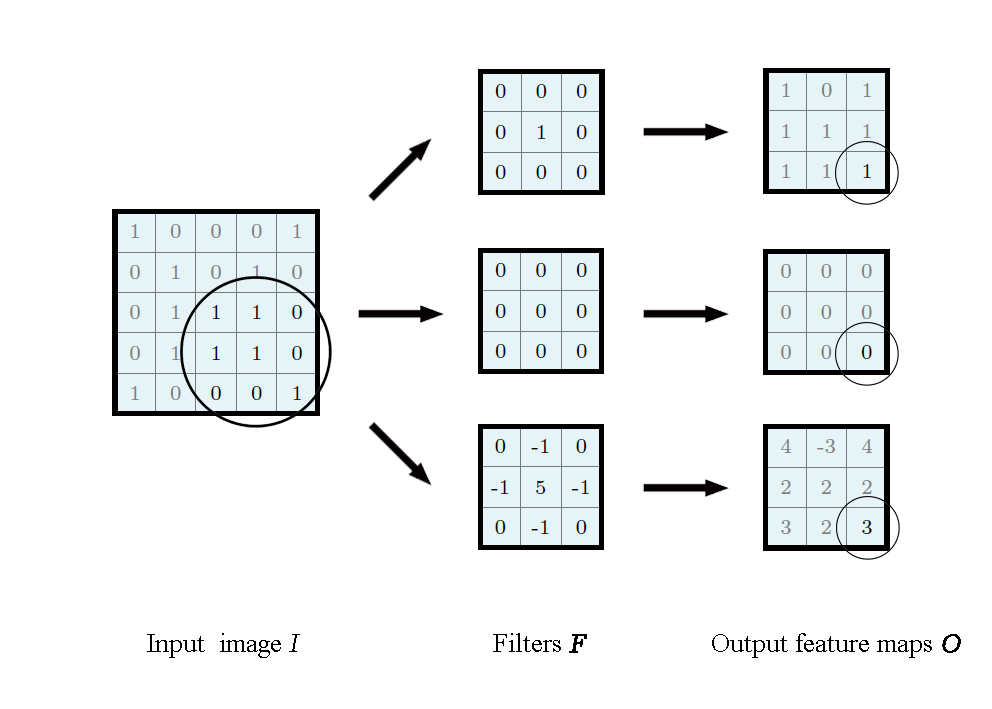
\includegraphics[scale=0.35]{p1b.png}
  \caption{Overall link between $I$ and $\pmb{O}$ with the bottom right pixels circled}
\end{figure}

\end{document}
